\subsection{Power laws and fat tails distributions}
Examine price records more closely, and you typically find a different kind of distribution than the bell curve: the tails follow a "\textbf{power law}". These are common in nature: if the sizes of the sides of a square doubles, the area quadruples, if the side triples, the area rises nine-fold; gravity weakens by the inverse power of two with the distance, ...\\

In 1962 Benoit Mandelbrot showed that positive and negative price movements follow power laws rather than normal distributions.
\begin{figure} [H]
    \centering
    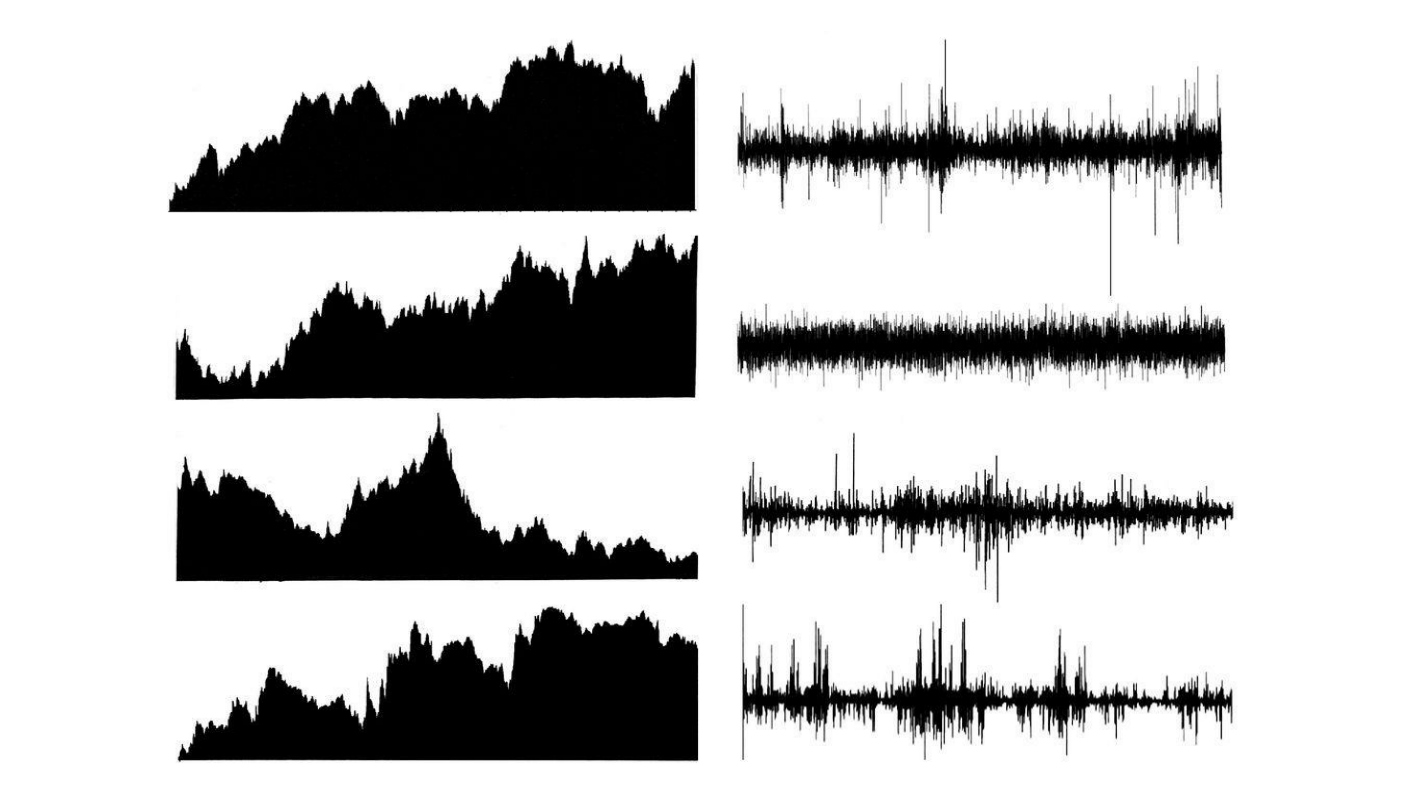
\includegraphics[width=1\linewidth]{img/market_comparison.jpg}
    \caption{On the left there are 4 price charts, the first and third are real chronicles, the second one is generated using classical models (BSM) and the last one is generated with one of the latest fractal and fat tails model. They pretty much look the same. To discover the differences one should look at the graph of the changes in logprice from moment to moment (shown on the left).}
    %\label{fig:placeholder}
\end{figure}
Power laws can be distributions with fat tails, meaning that the tail (the extreme values, the ones far from the mean) drops off more slowly than a thin tail (for example in the normal distribution).

An event 8 standard deviation from the mean:
\begin{itemize}
    \item In a normal distribution, it has a probability of $6 \cross 10^{-16}$;
    \item In a power law distribution, it can have a probability of almost $4 \%$, much higher.
\end{itemize}

Using a thin-tailed model for a fat-tailed phenomenon means underestimating risk of extreme events.
\begin{figure} [H]
    \centering
    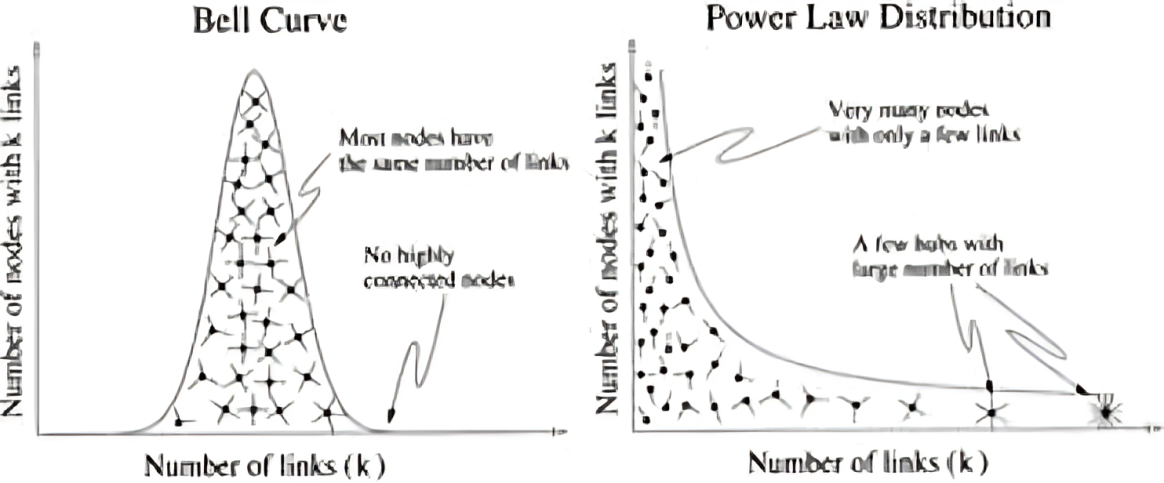
\includegraphics[width=1\linewidth]{img/ee.png}
    \caption{Normal distribution vs Power law Distribution.}
    %\label{fig:placeholder}
\end{figure}

\subsection{What are fractals?}
"\textit{A fractal is a rough or fragmented geometric shape that can be split into parts, each of which is (at least approximately) a reduced-size copy of the whole}" (Benoit Mandelbrot). \\

Among the features of a fractal we can find:
\begin{itemize}
    \item Self-similarity;
    \item Fine or detailed structure at arbitrarily small scales;
    \item Irregularity both locally and globally, that cannot easily be described with traditional Euclidean geometry without the use of recursion.
\end{itemize}
For example, a straight line is not a fractal, since it is self similar but it lacks detail and can be described with Euclidean geometry without the need for recursion.
\begin{figure} [H]
    \centering
    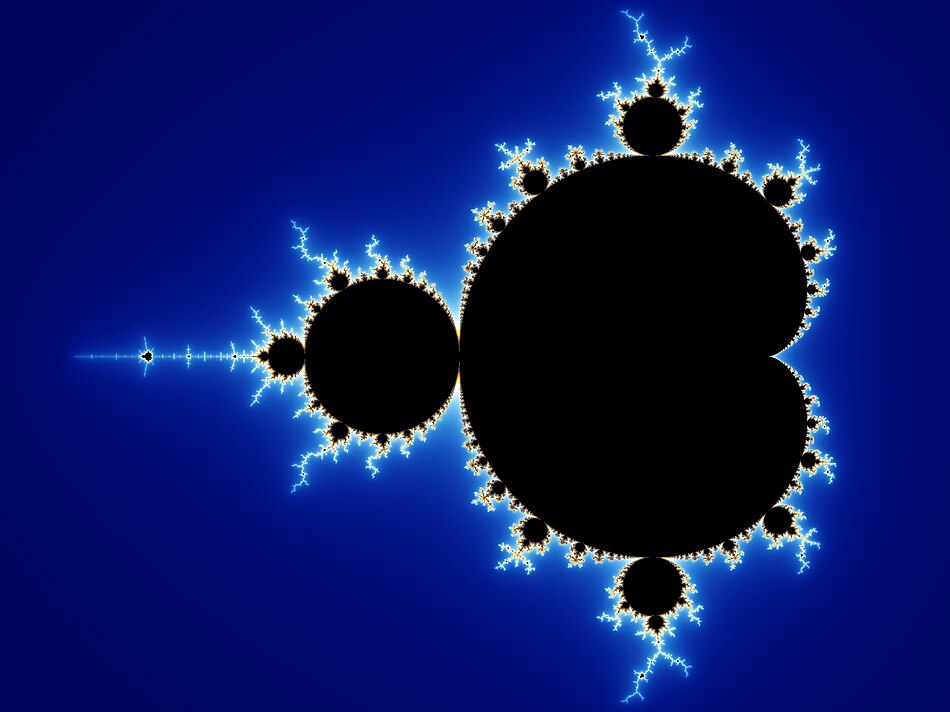
\includegraphics[width=0.65\linewidth]{img/Mandel_zoom_00_mandelbrot_set.jpg}
    \caption{The boundary of the Mandelbrot set is a fractal curve.}
\end{figure}
\subsection{Fractality in the finantial market}
\textbf{What evidence suggests that financial markets may exhibit fractal properties?}
\begin{itemize}
    \item When comparing the price charts and log-returns of different financial markets, it is very difficult to identify significant differences.
    \begin{figure} [H]
        \centering
        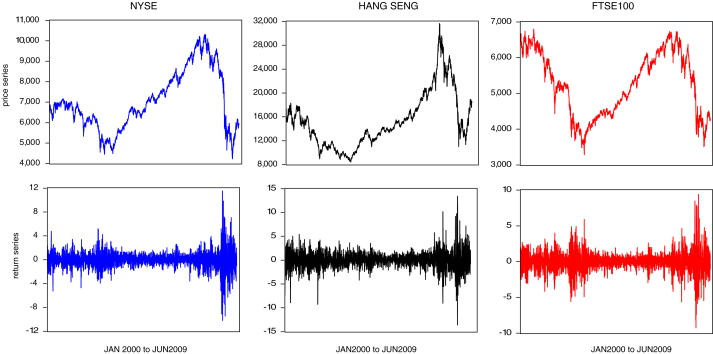
\includegraphics[width=1\linewidth]{img/fractal_1.png}
        \caption{There are very little differences in these three different finantial markets.}
    \end{figure}
    \item If we take the liberty of examining the price charts of the New York Stock Exchange (NYSE) while concealing the axis labels and applying suitable dilations or contractions along the vertical axis, it becomes impossible to distinguish one time scale from another—that is, whether we are observing price variations over the course of a single day or an entire year.

\begin{figure}[htbp]
    \centering
    % --- Prima riga ---
    \begin{subfigure}{0.45\textwidth}
        \centering
        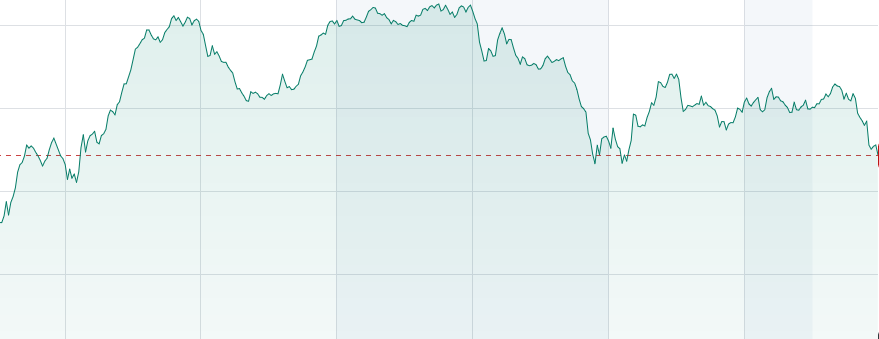
\includegraphics[width=\linewidth]{img/1d.png}
        \caption{Price over 1 day.}
    \end{subfigure}
    \hfill
    \begin{subfigure}{0.45\textwidth}
        \centering
        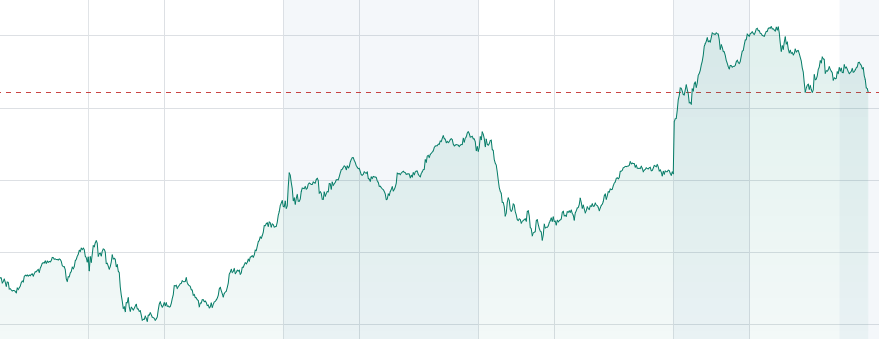
\includegraphics[width=\linewidth]{img/5d.png}
        \caption{Price over 5 days.}
    \end{subfigure}

    % --- Seconda riga ---
    \begin{subfigure}{0.45\textwidth}
        \centering
        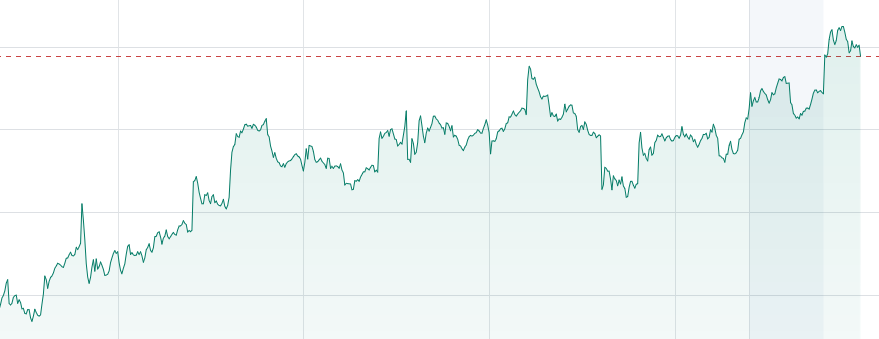
\includegraphics[width=\linewidth]{img/1m.png}
        \caption{Price over 1 month.}
    \end{subfigure}
    \hfill
    \begin{subfigure}{0.45\textwidth}
        \centering
        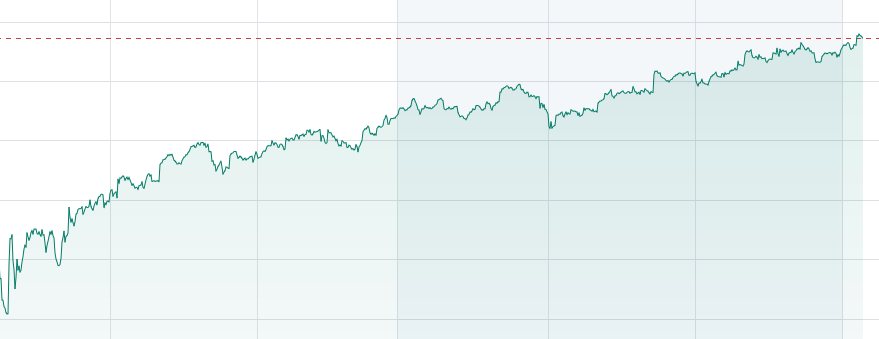
\includegraphics[width=\linewidth]{img/1y.png}
        \caption{Price over 1 year.}
    \end{subfigure}

    % --- Terza riga ---
    \begin{subfigure}{0.45\textwidth}
        \centering
        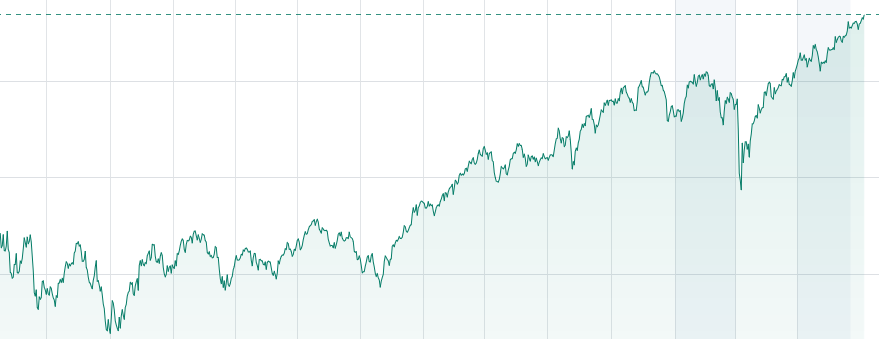
\includegraphics[width=\linewidth]{img/5y.png}
        \caption{Price over 5 years.}
    \end{subfigure}
    \hfill
    \begin{subfigure}{0.45\textwidth}
        \centering
        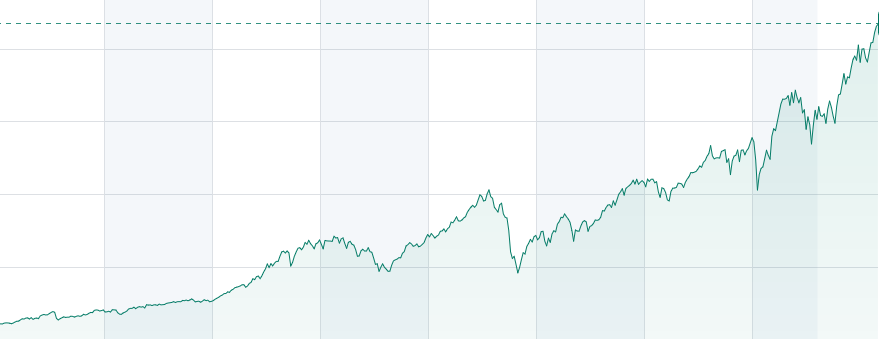
\includegraphics[width=\linewidth]{img/30y.png}
        \caption{Price over 30 years.}
    \end{subfigure}
        \caption{Prices of NYSE Composite Index at different time scales.}
    \label{fig:siximages}
\end{figure}
    It is evident from the simple experiment just carried out that financial markets exhibit \textbf{self~-~similarity} across different time scales and detailed structure at arbitrarily small scales.
\end{itemize}

\subsection{Chaos in the finantial market}
Another characteristic that helps explain the irregularity of financial markets is their \textbf{chaotic nature}. Sudden crashes, bursts of volatility, and persistent cycles suggest that markets may not be purely random, but rather governed by nonlinear dynamics that resemble chaotic systems.\\

Chaos does not imply complete disorder. Instead, it refers to systems that are deterministic in structure yet highly sensitive to initial conditions—a phenomenon widely known as the “Butterfly Effect.” This sensitivity makes long-term prediction practically impossible, even when the underlying rules are well defined.\\

As we will illustrate with an example in this chapter, the chaotic nature of financial dynamics can be detected in real BTC-USD price data.\\
In particular, we will find that the data follow an \textbf{attractor}, that is, a set of states toward which the system tends to evolve over time, regardless of small modifications to the initial conditions. Specifically, the attractor we will identify is a \textbf{strange attractor}, a hallmark of a chaotic system, since its fractal dimension is non-integer, thereby exhibiting self-similarity across different scales and trajectories that never repeat exactly, while still remaining within the basin of attraction.
\begin{figure} [H]
    \centering
    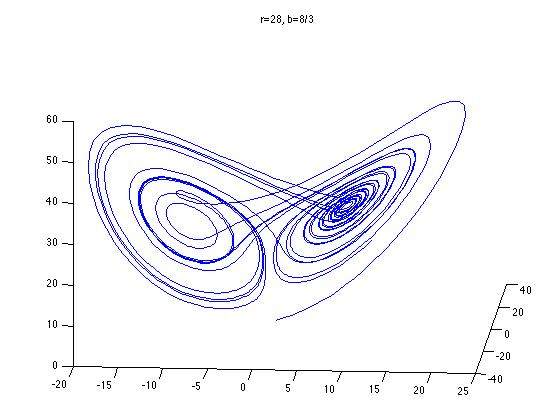
\includegraphics[width=0.75\linewidth]{img/image.png}
    \caption{A Lorentz attractor, a very well known example of strange attractor.}
\end{figure}

\subsection{Takens' Theorem: The importance of the Past in Reconstructing the future}
Having introduced the notion of strange attractors as the geometric signature of chaos, we are now in a position to ask how such structures can be uncovered from real data.\\

In practice, we rarely have access to the full set of equations governing a system; instead, we tipically observe only a \textbf{single time series}, such as a financial price.\\

\textbf{Takens' embedding theorem} (1981, Floris Takens) represents a cornerstone in the study of nonlinear dynamics and chaos.\\

At its core, the theorem demonstrates that it is possible to reconstruct the underlying structure of a dynamical system (even if it shows chaotic behavior) by observing only a single time series of measurements.\\

This justifies the use of \textbf{time-delay embedding methods} to forecast the behavior of chaotic systems such as financial markets. An example of these methods will be discussed in the following chapter.\\

A mathematically rigorous formulation of the theorem's statement would require advanced knowledge and would centainly fall beyond the scope of this review.\\

Nevertheless we can still grasp the general idea of the theorem, but since it is not essential for understanding the following chapters, what follows may be skipped:\\

\textit{Suppose we have a $d$-dimensional state vector $x_t$ that evolves according to an unkown but continuous and deterministic dynamic.} \textit{In simple terms, we require that the differential equations governing the system be continuous and deterministic. This is crucial, since if the system were purely stochastic, there would be no way to reconstruct its evolution.}\\
\textit{Suppose, too, that the one-dimensional observable $y$ is a smooth function of $x$, and coupled to all the components of $x$. In our case this $y$ may be the price at a given time.}\\

\textit{At any time we can look not just at the present measurement $y(t)$, but also at observations made at times removed from us by multiples of some lag $\tau$: $y_{t+\tau},t_{t+2\tau},...$.\\}
\textit{If we use $k$ lags, we will have a $k$-dimensional vector.\\}
\textit{As one might expect, in the limit $k \to \infty$ the motion on the lagged space becomes deterministic at a finite dimension; not only that, but this deterministic dynamics (in the lagged space) are equivalent to those of the original state space. (They are related by a smooth, invertible change of coordinates, or if you like it more a diffeomorphism.)}



\subsection{How fractals can explain the market? (k-NN method)}\label{sec:k-NN_method}
Many algorithms use fractals in an attempt to forecast market prices, let us now explore one of the most widely used algorithms, called the k-NN method (k-nearest neighbours), which exploits fractal dimension and lag points to account for the irregularities in past data, as justified by Takens's theorem.
\begin{itemize}
    \item \textbf{Make a lag plot of your price data}:\\
    Consider the price series $\{x_i,i=1,...,n\}$, to build a lag plot, you take this time series and plot each value against its lagged version. For example, if you choose a lag of 1, you plot the pairs $(x_i,x_{i-1})$.\\
The horizontal axis represents the lagged values, while the vertical axis represents the current values. By varying the lag length ($L$), you can explore how the present depends on past observations. If the points appear randomly scattered, the series has little temporal dependence; if patterns or structures emerge, this indicates correlations or nonlinear dynamics in the data.
    \item \textbf{Compute the fractal dimension:}\\
    Now we need to compute the fractal dimension of the time series in order to measure how the complexity of the data changes with scale. \\
    You can compute the fractal dimension with the \textbf{box-counting method}: \\

    Cover the whole set of points with $\varepsilon$-sized boxes (in our case you need to cover the points in the lag-plot with squares, 2-D boxes).\\
    Then count the number of boxes you used $N(\varepsilon)$ and take the limit $\varepsilon \to 0$ to get the box-dimension:
    \begin{equation*}
         f=\lim_{\varepsilon \rightarrow 0} \frac{\ln(N(\varepsilon))}{\ln(1/\varepsilon)}    
    \end{equation*}
    
    There are plenty of other algorithms that one may use to compute the fractal dimension of a set of points (as the correlation dimension explained in Appendix \ref{app:C_Correlation_dimension}).
    \item \textbf{Find the optimal lag length} $\boldsymbol{\tilde{L}}$:\\
    It is necessary to decide the lenght of the lag. If it is too short, the reconstructed space does not capture enough of the underlying structure; if it is too long, the representation becomes redundant and noisy.\\
    
    
    The lag length specifies the number of steps back in time that must be considered when constructing the pairs in the lag plot. \\
    For example if you have a lag length of $L=2$ the pairs of the lag plot are $(x_t,x_{t-2})$ \textit{(there's a generalisation to a multilag embedding that consider all the $L$ previous lagged values. So in the previous case the lag plot will be a 3-D plot with points $(x_t,x_{t-1},x_{t-2})$, and so on for higher values of $L$)}.\\

    
    A practical way to determine the optimal lag length ($\tilde{L}$) is to compute the fractal dimension of the lag plots for increasing lag values.\\
    You expect to see something like this:
    \begin{figure}[H]
        \centering
        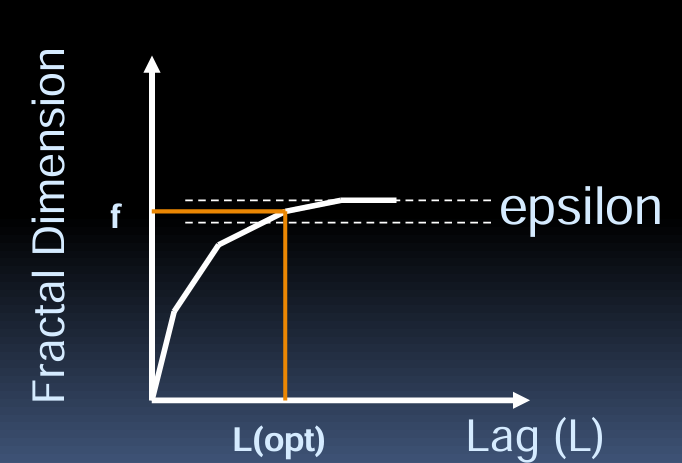
\includegraphics[width=0.6\linewidth]{img/image2.png}
        \caption{Fractal dimension of the lag plots for increasing lag values.}
        %\label{fig:placeholder}
    \end{figure}
    As the lag grows, the estimated fractal dimension will initially increase, since we are discovering new independent information. At some point, however, the dimension stabilizes within a fixed small tolerance ($\varepsilon$). The lag value at which this stabilization occurs is chosen as the optimal lag lenght $\tilde{L}$.\\

    
    (\textit{In the multi-lag embedding you can compute the fractal dimension by covering the $N$-dimensional plot with hyper-cubes})\\

    
    Basically what we have computed is the smallest number of past observations needed to capture the intrinsic complexity of the time series without adding unnecessary redundancy.
    \item \textbf{Optimal number of lag points:}\\
    The aim here is doing an interpolation whithin a set of nearest neighbors of the current point.\\
    But we need to choose the optimal number of neighbouring lag points $\tilde{k}$.\\
    If too few neighbors are selected, the interpolation becomes unstable and overly sensitive to noise: however if too many are included, the prediction is oversmoothed and loses the local structure of the dynamics. \\

    
    There's a conjecture proposing that the optimal number of neighbors is directly related to the fractal dimension $(f)$:
    \begin{equation*}
        \tilde{k} \sim  \mathcal{O}(f)
    \end{equation*}
    and more specifically, a prectical rule of thumb is given by: $\tilde{k}=2f+1$.


    The conjecture is of course meaningful:
    \begin{itemize}
        \item An higher fractal dimension $f$ indicates more irregularity whose local geometry  can only be captured with more neighbors;
        \item Conversely, a lower $f$ corresponds to smoother dynamics, where fewer neighbors are sufficient.
    \end{itemize}
    \item \textbf{Nearest Neighbours Interpolation:}\\
    We perform interpolation using the nearest neighbours, since we believe that similar past states tend to evolve in similar ways. 
    We need to reconstruct the lag plot (using $\tilde{L}$) and choose a distance metric (typically the Euclidean distance) to identify the $\tilde{k}$ nearest neighbours.

    Once the nearest neighbours are identified, their subsequent values (what their value have become) are collected and used to estimate the future of the current state.\\
    \\
\begin{figure} [H]
    \centering
    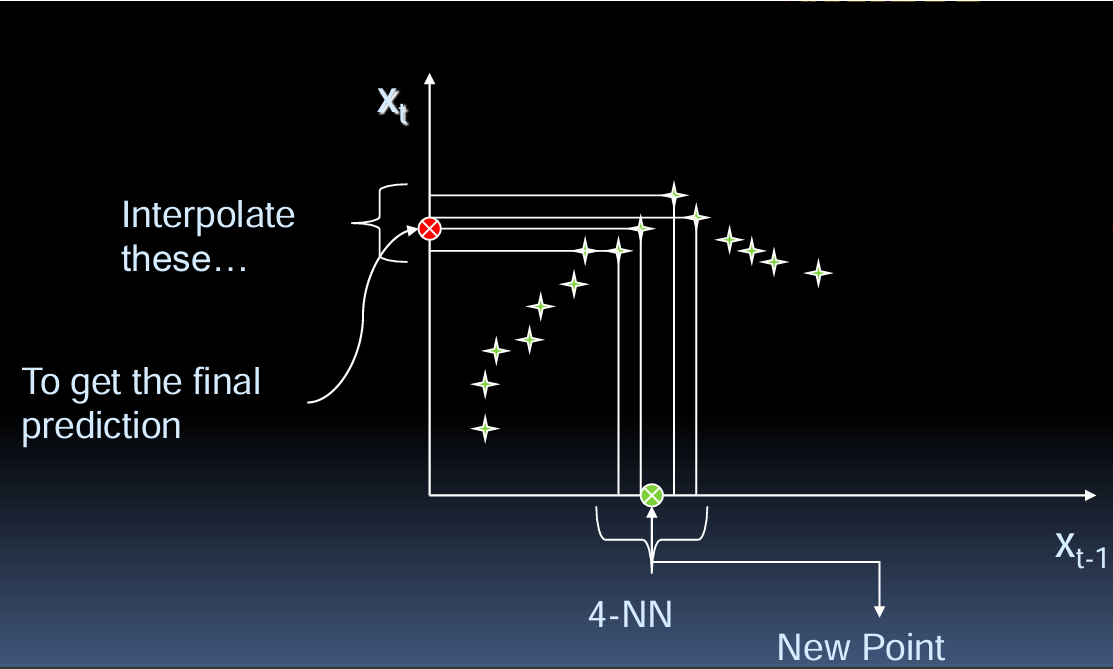
\includegraphics[width=0.75\linewidth]{img/interpolation.png}
    \caption{Nearest neighbours interpolation scheme.}
\end{figure}
    You can take the arithmetic mean of these future values, or you can take a weighted mean, with distance-based weights (giving greater importance to closer neighbours).
\end{itemize}

\subsection{Case study - Chaos in the Bitcoin price} \label{sec:Chaos_BTC}
Let us apply what we have discovered to the price of Bitcoin in US dollars from 2015 up to today.
\begin{itemize}
    \item \textbf{Calculation of the log-returns of the price series:}\\
        To analyze market dynamics, we first calculate the log returns of the price series, which is more suitable for chaos theory analysis:
    \begin{equation*}
        r_t = \ln\!\left(\frac{P_t}{P_{t-1}}\right)
    \end{equation*}
    \begin{figure}[H]
        \centering
        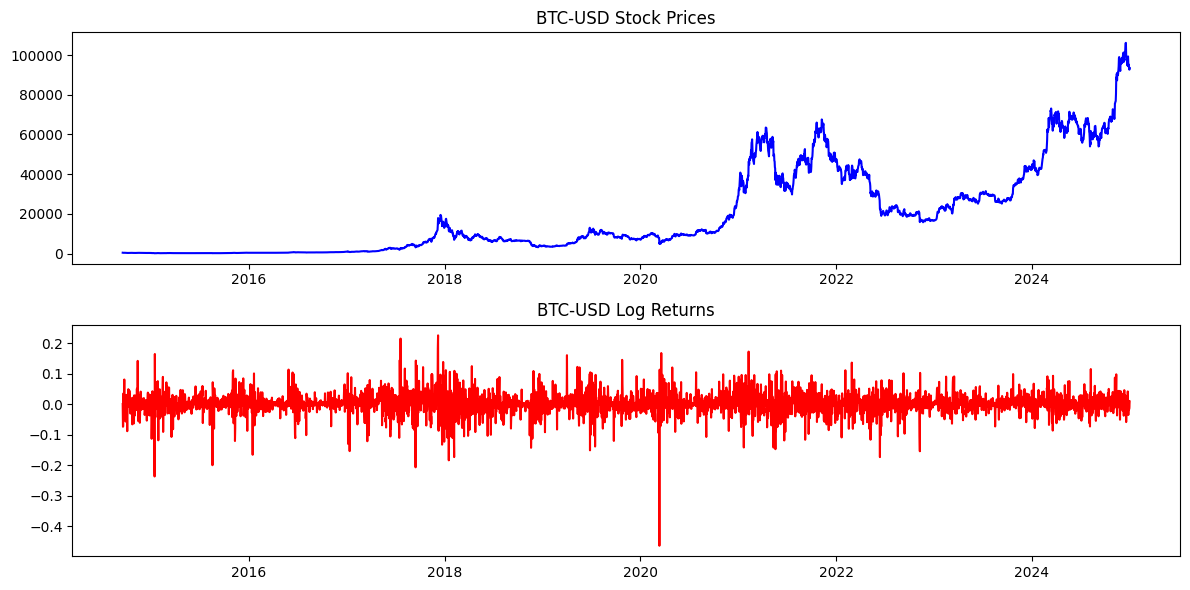
\includegraphics[width=1.00\linewidth]{img/bitcoin_prices.png}
        %\caption{Enter Caption}
    \end{figure}
    At first glance, the sharp decline of more than 40$\%$ in the BTC-USD price on March 12, 2020 is evident.
    
    \item \textbf{Constrution of the lag-plot:}\\
        We now construct the lag-plot (time-delay embedding) by plotting the log-returns against their past values, obtaining:
    \begin{figure}[H]
        \centering
        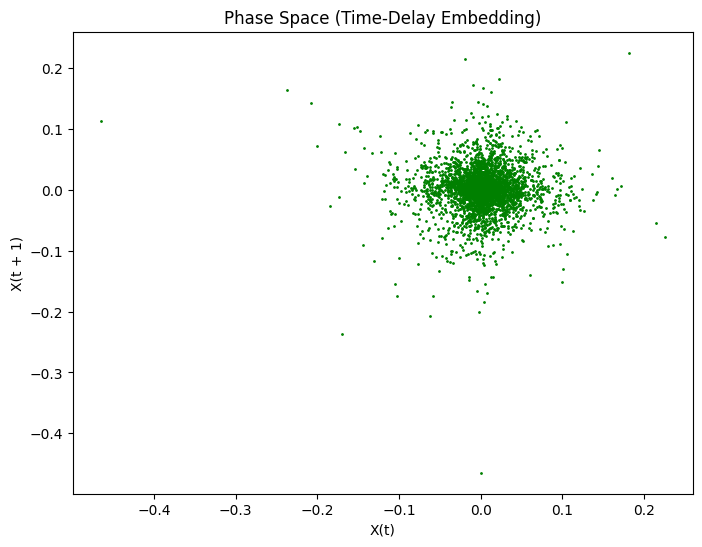
\includegraphics[width=0.75\linewidth]{img/lag_plot_bitcoin.png}
        \caption{Lag-plot of Bitcoin log-returns.}
    \end{figure}
    This plot represents a simple two-dimensional strange attractor. It shows how chaotic the stock return series behaves over time.
    
    \item \textbf{Calculation of the fractal dimension (correlation dimension):}\\
    We first compute the Euclidean distance between every pair of points in the previous lag-plot, thereby obtaining the distribution of separations between states. We then introduce a sequence of radii $\{r_i\}_i$ and for each radius value we count how many pair of points $C(r_i)$are closer than $r_i$. This produces a set of values $C(r)$ as a function of $r$, which can subsequently be represented o a log-log scale:


    \begin{figure}[H]
        \centering
        \begin{subfigure}[t]{0.49\textwidth}
            \centering
            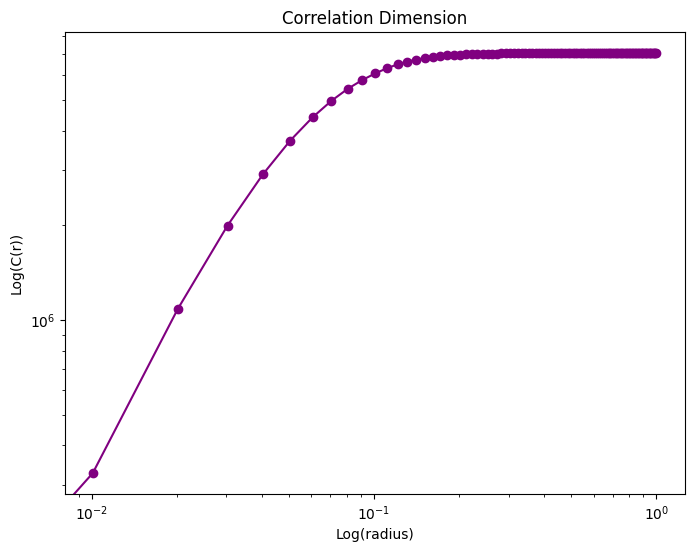
\includegraphics[width=\linewidth]{img/bitcoin_dimension.png}
            \label{fig:bitcoin_dimension}
        \end{subfigure}
        \hfill
        \begin{subfigure}[t]{0.49\textwidth}
            \centering
            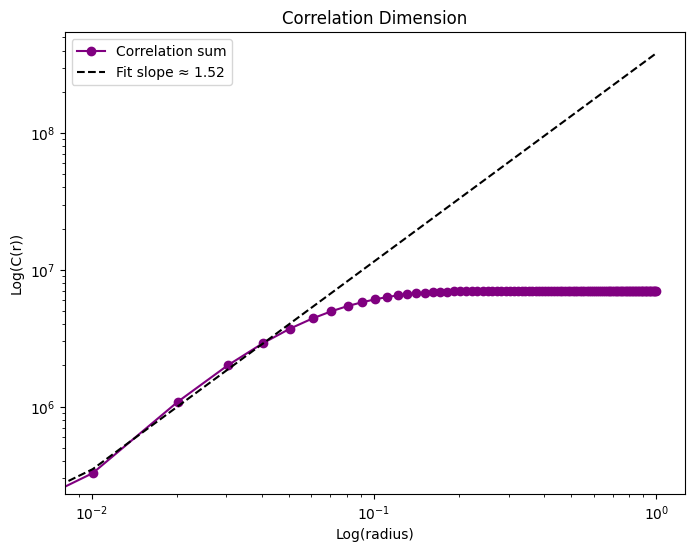
\includegraphics[width=\linewidth]{img/correlation_dimension.png}
            \label{fig:correlation_dimension}
        \end{subfigure}
        \caption{Estimation of Bitcoin’s correlation dimension.}
        \label{fig:dimension_estimation}
    \end{figure}
    
    As described in Appendix \ref{app:C_Correlation_dimension}, it is possible to estimate the correlation dimension (fractal dimension) by measuring the slope of the initial linear portion of the plot:
    
    So the estimated fractal dimension of the system is about $1.52$.
    
    A non-integer fractal dimension (such as $1.52$) is typical of chaotic attractors (strange attractors): it indicates that the system possesses a complex geometric structure, with trajectories that intertwine without ever repeating exactly.
    
    \item \textbf{BTC-USD price forecasts}\\
    Using the k-NN algorithm described in section \ref{sec:k-NN_method}, one can proceed to make BTC-USD price forecasts:
    \begin{figure} [H]
        \centering
        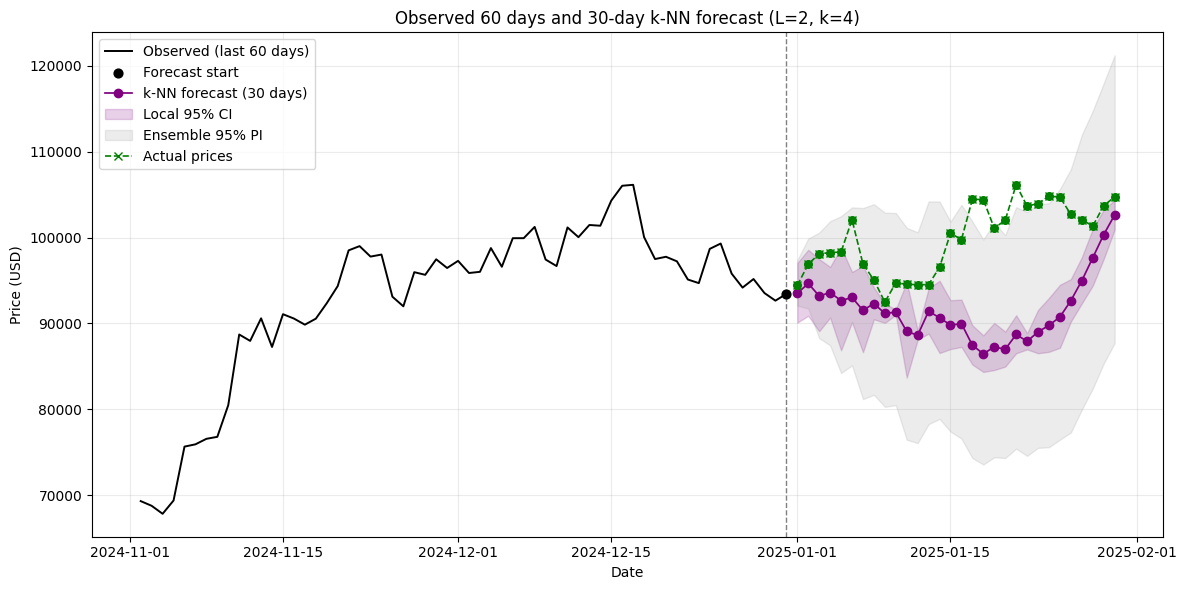
\includegraphics[width=1\linewidth]{img/forecast.png}
        \caption{Price over the last 60 days (black) and 30-day k-NN forecast (purple).}
    \end{figure}
    Here we plotted the prices for the last 60 days (black) and the 30-day ahead forecasts produced by the k-NN algorithm (in purple). The actual prices for January 2025 are shown in green.
    
    As shown in the chart, our forecasts closely track the actual prices only for the very first days, then match only the general trend. This should not surprise us since the algorithm is primarily designed to predict the next single price, and the observed discrepancy is merely further evidence of the system’s chaotic nature.\\
    \textit{(Some may view this as empirical evidence supporting the Efficient Market Hypothesis (EMH), but remember that we used a very simplistic algorithm, and far more complex and accurate methods exist that also make use of machine learning.)}
\end{itemize}